\chapter{Założenia projektowe}

\section{Wprowadzenie}

W niniejszym rozdziale przedstawiono założenia projektowe systemu NetHelt, opracowanego w ramach pracy inżynierskiej. Rozdział obejmuje opis przedmiotu pracy, wizję tworzonej aplikacji, wymagania funkcjonalne i niefunkcjonalne oraz zarys architektury logicznej i fizycznej systemu.

Celem przedstawionych założeń jest określenie sposobu realizacji systemu monitorowania urządzeń sieciowych działających w środowisku lokalnym. Opisane zostały zarówno wymagania dotyczące funkcjonalności aplikacji, jak również aspekty związane z bezpieczeństwem, wydajnością oraz komunikacją pomiędzy poszczególnymi modułami systemu.

Projektowany system ma charakter wielomodułowy i składa się z aplikacji webowej, aplikacji desktopowej działającej jako klient monitorujący oraz modułu analizy danych wykorzystującego algorytmy sztucznej inteligencji do wykrywania anomalii sieciowych. W rozdziale przedstawiono również ogólną koncepcję architektury rozwiązania oraz relacje pomiędzy jego komponentami.

Założenia opisane w dalszej części pracy stanowią podstawę do implementacji systemu oraz realizacji poszczególnych etapów projektu.

\section{Przedmiot pracy i wizja aplikacji}

Przedmiotem pracy jest opracowanie wielomodułowego systemu informatycznego do monitorowania urządzeń sieciowych działających w środowisku lokalnym (LAN). System ma umożliwiać kontrolę stanu urządzeń, analizę jakości połączenia sieciowego oraz wykrywanie anomalii mogących świadczyć o problemach w działaniu infrastruktury sieciowej.

Projektowane rozwiązanie składa się z aplikacji webowej, aplikacji desktopowej oraz modułu analizy danych wykorzystującego algorytm \texttt{Isolation Forest}. Aplikacja webowa odpowiada za zarządzanie systemem i prezentację danych użytkownikowi, natomiast aplikacja desktopowa realizuje operacje monitorujące w sieci lokalnej i przesyła wyniki do centralnego serwera.

System przewiduje obsługę użytkowników standardowych oraz administratorów, posiadających rozszerzone uprawnienia zarządzania systemem. Aplikacja ma umożliwiać m.in. konfigurację urządzeń, monitorowanie ich dostępności, analizę parametrów połączenia oraz wysyłanie powiadomień o wykrytych problemach.

Wizja projektu zakłada stworzenie skalowalnego i łatwego w rozbudowie systemu, dostępnego z poziomu przeglądarki internetowej oraz wdrożonego w środowisku chmurowym. Komunikacja pomiędzy modułami będzie realizowana z wykorzystaniem interfejsów API oraz centralnej bazy danych PostgreSQL.

\section{Wymagania funkcjonalne}

Wymagania funkcjonalne określają funkcje oraz operacje, które system powinien realizować z perspektywy użytkownika. Ich celem jest opisanie zachowania aplikacji oraz możliwości udostępnianych poszczególnym aktorom systemu. 

W procesie analizy wymagań wykorzystano koncepcję \emph{user stories}, stosowaną w metodykach zwinnych do opisu oczekiwań użytkowników wobec systemu \cite{www2}. Na podstawie przeprowadzonej analizy opracowano zestaw wymagań funkcjonalnych dla projektowanej aplikacji.

W systemie wyróżniono trzech głównych aktorów:
\begin{itemize}
	\item administratora,
	\item użytkownika,
	\item gościa.
\end{itemize}

Administrator posiada uprawnienia do zarządzania użytkownikami oraz konfiguracją systemu. Użytkownik może zarządzać własnymi urządzeniami i konfiguracją monitorowania. Gość jest niezalogowanym użytkownikiem aplikacji i posiada dostęp wyłącznie do podstawowych funkcji systemu.

Zestaw wymagań funkcjonalnych przedstawiono w tabeli \ref{tab:functional-requirements}.

\begin{table}[H]
	\centering
	\caption{Wymagania funkcjonalne systemu}
	\label{tab:functional-requirements}
	\vspace{10pt}
	
	\begin{tabular}{p{1cm} p{12cm}}
		\toprule
		ID & User Story \\
		\midrule
		
		F-G1 & Jako gość, chcę zobaczyć informację na temat aplikacji, aby zrozumieć jej przeznaczenie \\
		F-G2 & Jako gość, chcę się zarejestrować, aby uzyskać dostęp do sytemu \\
		F-G3 & Jako gość, chcę się zalogować, aby korzystać z funkcji systemu \\
		F-G4 & Jako gość, chcę zresetować hasło, aby odzyskać dostęp do konta \\
		F-U1 & Jako użytkownik, chcę dodać urządzenie, aby je monitorować \\
		F-U2 & Jako użytkownik, chcę przeglądać listę swoich urządzeń, aby mieć wgląd w ich stan \\
		F-U3 & Jako użytkownik, chcę usunąć urządzenie, aby utrzymać porządek \\
		F-U4 & Jako użytkownik, chcę edytować dane urządzenia, aby zachować aktualność informacji \\
		F-U5 & Jako użytkownik, chcę konfigurować powiadomienia, aby otrzymywać informację na bieżąco  \\
		F-U6 & Jako użytkownik, chcę przeglądać statystyki moich urządzeń, aby w łatwy sposób kontrolować czasy odpowiedzi \\
		F-U7 & Jako użytkownik, chcę pobrać klienta desktopowego, aby skonfigurować połączenie w mojej sieci  \\
		F-U8 & Jako użytkownik, chcę zmienić swoje hasło, aby zachować bezpieczeństwo konta \\
		F-U9 & Jako użytkownik, chcę się wylogować, aby zablokować nieautoryzowany dostęp do mojego konta \\
		F-A1 & Jako administrator, chcę przeglądać listę użytkowników, aby mieć wgląd w konta w systemie \\
		F-A2 & Jako administrator, chcę usuwać i przywracać konta, aby zapewnić bezpieczeństwo systemu \\
		F-A3 & Jako administrator, chcę zmieniać role użytkowników, aby kontrolować ich uprawnienia \\
		F-A4 & Jako administrator, chcę resetować hasła użytkowników, aby umożliwić odzyskanie dostępu \\
		F-A5 & Jako administrator, chcę ręcznie wywoływać zadania z harmonogramu, aby mieć większą kontrolę nad przebiegiem działania aplikacji \\
		F-A6 & Jako administrator, chcę przeglądać ilość aktywnych użytkowników w danym okresie, aby być świadomym poziomu sukcesu aplikacji \\
		
		\bottomrule
	\end{tabular}
	
	\vspace{10pt}
	\small Źródło: opracowanie własne.
\end{table}

\section{Wymagania niefunkcjonalne}

Wymagania niefunkcjonalne określają ograniczenia oraz cechy jakościowe systemu informatycznego. W przeciwieństwie do wymagań funkcjonalnych nie opisują one konkretnych funkcji aplikacji, lecz definiują sposób działania systemu, jego wydajność, bezpieczeństwo, niezawodność oraz dostępność \cite{www3}. 

Wymagania niefunkcjonalne mają istotny wpływ na jakość projektowanego rozwiązania oraz komfort korzystania z systemu przez użytkowników. Ich analiza została przeprowadzona na podstawie literatury z zakresu inżynierii oprogramowania oraz założeń projektowych aplikacji \cite{ks1}.

Najważniejsze wymagania niefunkcjonalne projektowanego systemu przedstawiono w tabeli \ref{tab:nonfunctional-requirements}.

\begin{table}[H]
	\centering
	\caption{Wymagania niefunkcjonalne systemu}
	\label{tab:nonfunctional-requirements}
	\vspace{10pt}
	
	\begin{tabular}{p{3cm} p{10cm}}
		\toprule
		Kategoria & Wymaganie \\
		\midrule
		
		Wydajność & System powinien obsługiwać minimum 100 równoczesnych użytkowników \\
		
		Wydajność & Czas odpowiedzi API powinien być krótszy niż 500 ms dla 95\% zapytań \\
		
		Wydajność & System powinien wykorzystywać mechanizm cache’owania najczęściej używanych danych w celu redukcji czasu odpowiedzi o co najmniej 30\% \\
		
		Wydajność & Moduł AI powinien przetwarzać jednominutowe okno danych pojedynczego urządzenia w czasie krótszym niż 100 ms \\
		
		Dostępność & System powinien być dostępny przez minimum 99\% czasu w skali miesiąca \\
		
		Dostępność & Maksymalny jednorazowy czas niedostępności systemu nie powinien przekraczać 1 godziny \\
		
		Bezpieczeństwo & System powinien wykorzystywać autoryzację użytkownika opartą o JWT oraz OAuth2 \\
		
		Bezpieczeństwo & Komunikacja pomiędzy klientem a serwerem powinna być szyfrowana z wykorzystaniem protokołu HTTPS \\
		
		Bezpieczeństwo & Hasła użytkowników powinny być przechowywane w postaci skrótu kryptograficznego z wykorzystaniem algorytmu Argon2 \\
		
		Niezawodność & System powinien zapisywać logi błędów oraz umożliwiać ich przeglądanie administratorowi \\
		
		Niezawodność & System powinien posiadać mechanizm ponawiania połączeń z urządzeniami obejmujący minimum 3 próby \\
		
		\bottomrule
	\end{tabular}
	
	\vspace{10pt}
	\small Źródło: opracowanie własne.
\end{table}

\section{Zarys architektury}

Architektura systemu została zaprojektowana w sposób warstwowy, zgodnie z podejściem opisywanym przez R.C. Martina, które zakłada separację logiki biznesowej od szczegółów implementacyjnych oraz infrastruktury systemowej \cite{ks2}. Takie podejście umożliwia utrzymanie wysokiej spójności systemu oraz ułatwia jego dalszy rozwój i testowanie.

\subsection{Architektura logiczna}

Architektura logiczna opisuje strukturę systemu z perspektywy jego komponentów funkcjonalnych oraz relacji między nimi, niezależnie od środowiska uruchomieniowego. Koncentruje się na podziale odpowiedzialności oraz przepływie danych pomiędzy modułami.

System został podzielony na następujące elementy logiczne:
\begin{itemize}
	\item Frontend (aplikacja webowa),
	\item Backend (REST API + WebSocket),
	\item Moduł AI,
	\item Baza danych,
	\item Cache,
	\item Klient desktopowy.
\end{itemize}

Elementy te zostały zorganizowane w trzy warstwy:
\begin{itemize}
	\item warstwa prezentacji,
	\item warstwa logiki aplikacyjnej,
	\item warstwa danych.
\end{itemize}

Warstwa prezentacji obejmuje frontend oraz klienta desktopowego, które odpowiadają za interakcję z użytkownikiem. Warstwa logiki obejmuje backend oraz moduł AI, które realizują przetwarzanie żądań, logikę biznesową oraz analizę danych. Warstwa danych obejmuje bazę danych oraz mechanizm cache, odpowiedzialne za przechowywanie danych w sposób trwały oraz tymczasowy.

Komunikacja pomiędzy komponentami przebiega w następujący sposób:
frontend komunikuje się z backendem poprzez REST API oraz WebSocket, zapewniając komunikację w czasie rzeczywistym, natomiast klient desktopowy wykorzystuje REST API. Backend przetwarza żądania i deleguje zadania do modułu AI w celu analizy danych, a następnie zapisuje lub odczytuje dane z warstwy danych.

\begin{figure}[H]
	\centering
	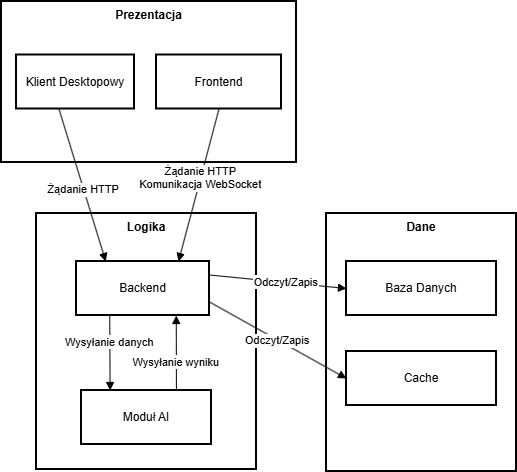
\includegraphics[width=0.8\textwidth]{images/logic-arch.jpg}
	\caption{Architektura logiczna systemu\\Źródło: opracowanie własne}
	\label{fig:logic-arch}
\end{figure}

\subsection{Architektura fizyczna}

Architektura fizyczna przedstawia sposób wdrożenia systemu w środowisku infrastrukturalnym. System został zaimplementowany z wykorzystaniem platformy Google Cloud Platform (GCP), która zapewnia skalowalne środowisko uruchomieniowe oraz usługi zarządzane.

Poszczególne komponenty systemu zostały skonteneryzowane przy użyciu technologii Docker. Każdy główny moduł działa w osobnym kontenerze, co zapewnia ich izolację oraz możliwość niezależnego wdrażania.

W warstwie fizycznej system obejmuje:
\begin{itemize}
	\item backend uruchamiany w kontenerze Docker,
	\item frontend uruchamiany w kontenerze Docker,
	\item moduł AI uruchamiany w kontenerze Docker,
	\item bazę danych realizowaną w usłudze Cloud SQL,
	\item cache realizowany w usłudze Memorystore,
	\item klienta desktopowego instalowanego lokalnie na urządzeniu użytkownika.
\end{itemize}

Takie podejście zapewnia separację komponentów, łatwość skalowania oraz zwiększoną odporność systemu na awarie, a także upraszcza proces wdrażania i utrzymania infrastruktury.

\begin{figure}[H]
	\centering
	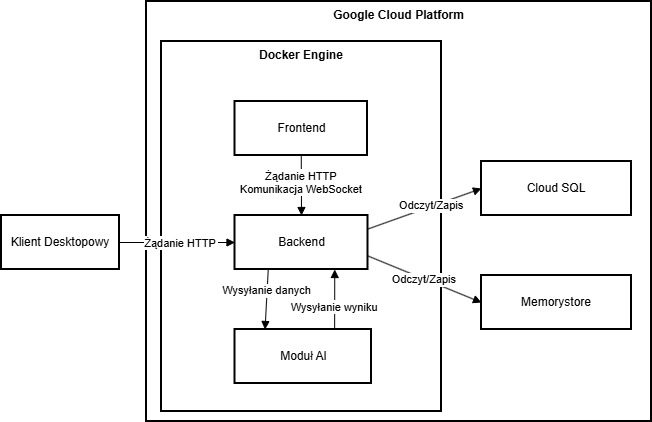
\includegraphics[width=0.8\textwidth]{images/physic-arch.jpg}
	\caption{Architektura fizyczna systemu\\Źródło: opracowanie własne}
	\label{fig:physic-arch}
\end{figure}